\chapter{[SKE] TTT transformace a plot, optimální preventivní údržba, model proporcionálních rizik.}

% lecture 5

\section{TTT transformace}

    \begin{define}[TTT transformace]
    Mějme veličinu $T\sim F$ takovou, že $\mu<+\infty$. Definujeme TTT transformaci vztahem $$ \HF(v)=\int_{0}^{F^{-1}(v)}\RT(t)\d t,\quad v\in[0,1],\quad F^{-1}(0)=0,\quad F^{-1}(1)=x_F,$$
    kde $x_F$ je pravý krajní bod rozdělení $F$.
    \end{define}

    \begin{remark}
        Spojení $F_T$ a $\HF$ je jednoznačné, t.j. pro každou $\HF$ existuje právě jedna $F_T$ a naopak. To sice umožňuje i $\RT$ apod., ale třeba pro Weibulla a exponenciální rozdělení bude mít $\HF$ výhodný tvar.
        Dále platí, že $$ \HF(1) = \int_{0}^{x_F}\RT(t)\d t=\int_{0}^{+\infty}\RT(t)\d t=\mu. $$
    \end{remark}

    \begin{define}[Škálovaná TTT transformace]
        Definujeme škálovanou TTT transformaci jako $\phi_F(v)=\frac{\HF(v)}{\mu}$.
    \end{define}

    \begin{figure}[h]
        \centering
        \includegraphics[width=0.4\linewidth]{pictures/TTT}
        \caption{Schéma $\HF$.}
        \label{fig:TTT}
    \end{figure}


    % lecture 6

    \begin{theorem}
        Mějme $F$ spojitou a ostře rostoucí. Pak pro $\forall t\in\big(0,F^{-1}(1)\big)$ platí, že $$\frac{\d}{\d v}\HF(v)\Big|_{v=F(t)}=\frac{1}{\lambda_T(t)}.$$
    \end{theorem}

    Pokud $\lambda_T(t)$ je rostoucí, pak $\frac{1}{\lambda_T(t)}$ je klesající a naopak. Klesající první derivace značí konkávnost $\HF$.

    \begin{define}[Empirická TTT transformace]
        Pro $\textbf{T}:=(T_1,...,T_n)~iid~F$ definujeme \textbf{Empirickou TTT transformaci} jako
        $$ H_n^{-1}(v):=\int_{0}^{F_n^{-1}(v)}\big(1-F_n(t)\big)\d t,\quad \phi_n(v)=\frac{H_n^{-1}(v)}{H_n^{-1}(1)}. $$
    \end{define}

    \begin{theorem}
        Platí, že $\inv{H_n}\rightrightarrows \inv{H_F}(v)$.
    \end{theorem}

    \begin{define}[TTT plot]
        Definujeme \textbf{TTT plot} jako graf $\Big\{\frac{i}{n},\phi_n\big(\frac{i}{n}\big)\Big\}_0^n$.
    \end{define}

    \begin{figure}[h]
        \centering    
        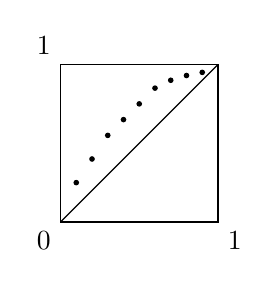
\begin{tikzpicture}[scale=2]
            \draw (0,0) -- (0,1) -- (1,1) -- (1,0) -- cycle;
            \draw (0,0) -- (1,1);
            
            \filldraw (0.1,0.25) circle (.4pt);
            \filldraw (0.2,0.4) circle (.4pt);
            \filldraw (0.3,0.55) circle (.4pt);
            \filldraw (0.4,0.65) circle (.4pt);
            \filldraw (0.5,0.75) circle (.4pt);
            \filldraw (0.6,0.85) circle (.4pt);
            \filldraw (0.7,0.9) circle (.4pt);
            \filldraw (0.8,0.93) circle (.4pt);
            \filldraw (0.9,0.95) circle (.4pt);
            
            \draw [color=black](0,0) node[anchor=north east] {0};
            \draw [color=black](0,1) node[anchor=south east] {1};
            \draw [color=black](1,0) node[anchor=north west] {1};
        \end{tikzpicture}
        \caption{Body jsou mimo diagonálu, takže to nejspíě neodpovídá exponenciálnímu rozdělení. Vidíme ale konkávní závislost, proto můžeme zkusit např. Weibulla. Snažíme se najít model, který se nejvíce přibližuje datům.} 
        \label{ttt-plot}
    \end{figure}

    \begin{remark}
        TTT plot se tak jmenuje, protože $$\inv{H_n}\Big(\frac{i}{n}\Big)\equal{...}\frac{1}{n}\Big[\sum_{j=1}^i t_{(j)}+(n-i)t_{(i)}\Big],$$ kde obsahu hranaté závorky se říká \textbf{Total test in time} v bodě $t_{(i)}$ (od $i$-té součástky počítáme pouze $t_{(i)}$, protože všechny byly v testu po dobu $t_{(i)}$). Test nutně nemusí skončit v době poruchy některé součástky, a tedy můžeme zavést symbol $\tau(t):=\sum_{j=1}^it_{(j)}+(n-i)t$, kde $T_{(i)}<t<T_{(i+1)}$.
    \end{remark}

\section{Preventivní údržba}

    Představme si třeba převodovku automobilu, kde jedna z komponent, klínový řemen, sice stojí pár korun ($c$), ale porucha řemene kompletně zničí celou převodovku, což se může prodražit ($c\ll k$). V této části se tedy pokusíme optimalizovat maintenance policy tak, aby se snížily náklady na provoz automobilu. Ještě vyšší potřeba je kontrola komponent u jaderných elektráren, kde je potřeba dělat odstávky a vyměnit všechny potřebné součásti tak, aby se minimalizovala pravděpodobnost havárie.

    Celkové náklady v čase $t$ se tedy spočítají jako $\sum_{\text{plán}}c+\sum_{\text{poruchy}}(c+k)$. Střední náklady na výměnnou periodu $t_0$ jsou tedy rovny $c+k\PP(T\leq t_0)$.
    
   \begin{define}[Střední náklady za jednotku času]
        Definujeme \textbf{střední náklady za jednotku času} $C_A(t_0)=\frac{c+k\PP(T\leq t_0)}{\mathrm{MTBR}(t_0)}$ pro Mean Time Before Replacement ve tvaru \[
    \begin{split}
        \mathrm{MTBR}(t_0)&=\E\bigg(Z(T)=\begin{cases}
            T,& T\leq t_0,\\ t_0,& T>t_0
        \end{cases}\bigg)=\int_{0}^{t_0}tf_T\d t+\int_{t_0}^{+\infty}t_0 f_T(t)\d t\equal{PP} \\ &= \int_{0}^{t_0\stackrel{!}{=}\inv{F}(v_0)}\big(1-F(t)\big)\d t=\HF(v_0),
    \end{split}
    \]
    kde jsme plynule přešli od $t_0$ k proměnné $v_0$.
    \end{define}
    
    Chceme $t_0$ optimalizovat tak, aby se minimalizovala veličina 
    $$C_A(v_0)=\frac{c+k\overbrace{F(t_0)}^{v_0}}{\HF(v_0)}=\frac{c+kv_0}{\mu\phi_F(v_0)}.$$ 
    Po derivaci úpravou dostaneme 
    $$ C_A'(v_0)=\frac{k\phi_F(v_0)-(c+kv_0)\phi_F'(v_0)}{\phi_F^2(v_0)}=0\quad\Rightarrow\quad \frac{\phi_F'}{\phi_F}=(\ln \phi_F)'=\frac{k}{c+kv_0}.$$

    Vyřešením této diferenciální rovnice dostaneme optimální $v_0$ (ne vždy ale máme $\phi_F$ a jsou tam i další problémy).

\section{Coxův Model Proporcionálních rizik}

    Doba do poruchy $T$ je ovlivněna doprovodnými vysvětlujícími faktory $\bold{X} =  (\bold{X}_1, \bold{X}_2,\dots, \bold{X}_q)$. Můžou to být kategorické proměnné - kouří/nekouří, nebo se může jednat i o spojitou proměnnou. Coxův model předpokládá tvar inzenzity poruch jako
    $$ r_T(t,\bold{X}) = r_0(t) \cdot \psi(\bold{X}, \boldsymbol{\beta}).$$
    Pokud dosadíme $\psi(\bold{X}, \boldsymbol{\beta}) = \e{\boldsymbol{\beta}\bold{X}} $ a zlogaritmujeme, tak získáme zobecněnou regresní úlohu
    $$\ln r_T(t) = \ln r_0(t) + \boldsymbol{\beta}\bold{X}. $$
    Tento tvar volíme, abychom věděli, kolikrát je např. placebo účinější, než zkoumaný lék.
    Snažíme se namodelovat výše zmíněnou závislost, odhadujeme regresní parametry. Tyto parametry však odhadujeme za přítomnosti RC censorovaných dat. Nesmíme u toho zapomenout, že naše forma dat je $(T_j, \delta_j)_{j=1}^n$. 
    
   \begin{define}[Hazard ratio]
    Definujeme hazard ratio jako
    $$ \mathrm{HR(\bold{X}_1, \bold{X}_2)} = \frac{r_T(t, \bold{X}_1)}{r_T(t, \bold{X}_2)} = \frac{\psi_1}{\psi_2} = \e{\sum_{k=1}^{q} \beta_k(X_k^{(1)}- X_k^{(2)})} = \e{\beta_1}.$$
    \end{define}
    
    Pro odhad parametrů $\boldsymbol{\beta}$ se používá tzv. částečný věrohodnostní odhad (partial ML)
    $$L_p(\boldsymbol{\beta})  =\prod_{j\in D } \frac{\psi(\bold{X}_{(j)}, \boldsymbol{\beta})}{\sum_{k \in \mathfrak{R}(t_{(j)})}\psi(\bold{X}_{(k)}, \boldsymbol{\beta})},$$
    ze kterého pak získáme
    $$ \widehat{\boldsymbol{\beta}}_\mathrm{PML} = \argmax L_p(\boldsymbol{\beta}).$$


